\chapter{Considerações Finais}


\section{Sobre o Trabalho}
%------------------------------------------------------------------------------%


\subsection{Cronograma} 
O Trabalho de Conclusão de Curso foi planejado, em longo prazo, em quatro ciclos 
de desenvolvimento de vinte e um dias cada um. As figuras \ref{cronograma} e 
\ref{gantt}, que foram extraídas da ferramenta OpenProj\footnote{Documentação e 
\textit{download} disponível em 
\url{http://sourceforge.net/projects/openproj/}}, apresentam o cronograma geral 
e o gráfico de Gantt do presente trabalho.

\begin{figure}[h]
\centering
	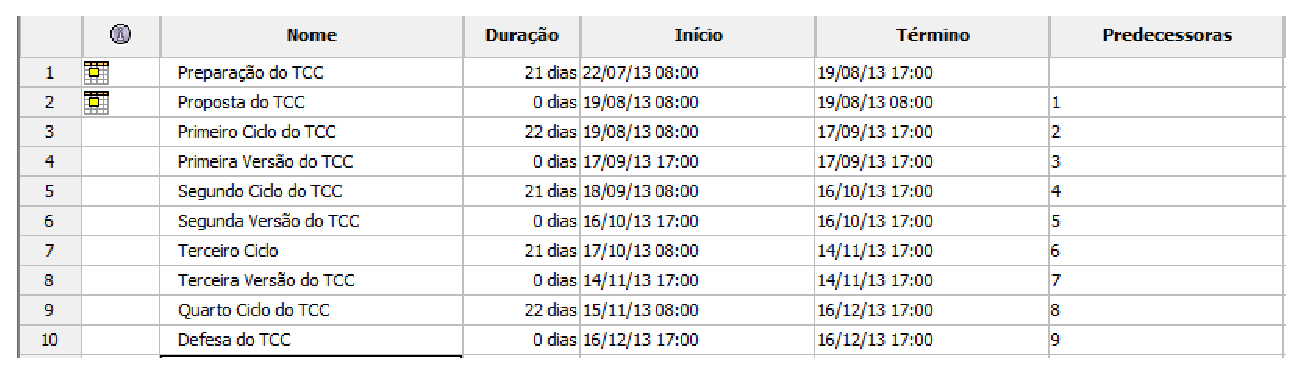
\includegraphics[keepaspectratio=true,scale=0.7]{figuras/marcos.eps}
	\caption{Ciclos de Desenvolvimento do Trabalho de Conclusão de Curso}
	\label{cronograma}
\end{figure}


\begin{figure}[h]
\centering
	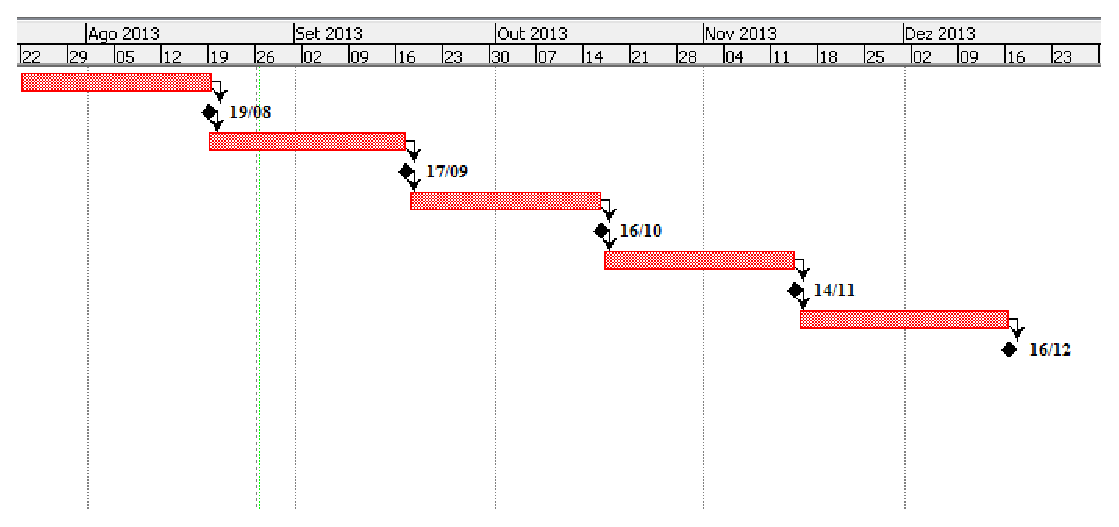
\includegraphics[keepaspectratio=true,scale=0.7]{figuras/gantt_chart.eps}
	\caption{Gráfico de \textit{Gantt} do Trabalho de Conclusão de Curso}
	\label{gantt}
\end{figure}

Para cada ciclo de desenvolvimento do Trabalho de Conclusão de Curso,  
utilizou-se o Quadro \textit{Kanban} para controle das atividades. 
O termo \textit{kanban} vem do japonês e significa literalmente "cartão de 
sinalização". O quadro \textit{kanban}, surgiu na Toyota, como um meio visual 
para controlar o fluxo da produção, limitando o tamanho do trabalho em progresso 
\cite{moura1999kanban}.

Posteriormente, o método foi incorporado no processo de desenvolvimento de
software pela metodologia ágil, \textit{Scrum} \cite{Schwaber:2004}. O quadro
\textit{Kanban} que foi utilizado no presente trabalho, foi criado na ferramenta 
\textit{online}, \textit{Kanban Flow}\footnote{Disponível em
\url{https://kanbanflow.com}}, e foi dividido em três colunas: 
\textbf{Backlog}, que são tarefas a fazer, \textbf{Em Progresso}, que são 
tarefas iniciadas e \textbf{Concluído} que mostra as tarefas que já foram 
executadas. A figura \ref{kanban} mostra o \textit{Kanban} ao final do segundo 
ciclo de desenvolvimento.

\begin{figure}[h]
\centering
	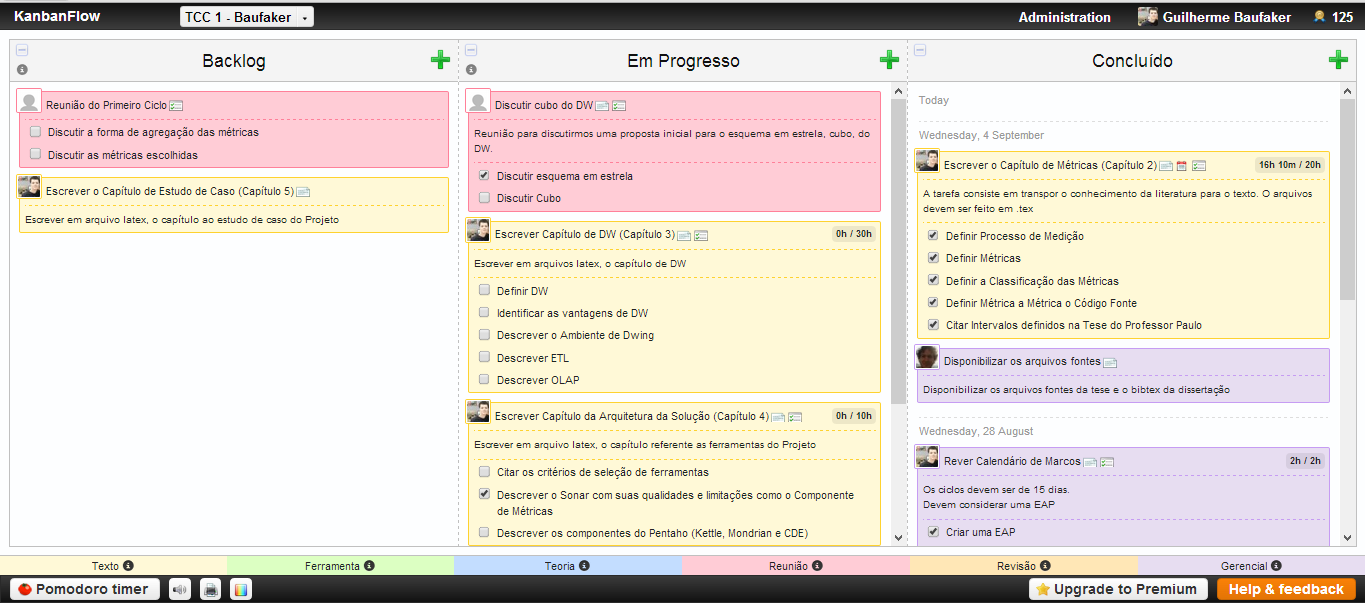
\includegraphics[keepaspectratio=true,scale=0.40]{figuras/kanban.eps}
	\caption{Quadro \textit{Kanban} do Trabalho de Conclusão de Curso}
	\label{kanban}
\end{figure}

\subsection{Considerações Finais}

\subsection{Trabalhos Futuros}
